\section{Reducción de dimensiones}

\subsection{Introducción}

Disponemos de un dataset de Bag of Words (BOW) que representan descripciones de texto correspondientes a compañías Brasileras clasificadas en nueve categorías distintas. Cada BOW contiene 856 atributos correspondientes a frecuencias de palabras y, debido a la alta dimensionalidad, se busca reducir el conjunto de datos a 3 dimensiones mediante las reglas de aprendizaje de Oja y Sanger.

Regla Oja:
\begin{itemize}
	\item$\Delta W_{ij} = \eta (x_i - \widetilde{x_i}) y_j$
	\item$\widetilde{x_i} = \sum_{j=1}^m y_j . W_{ij}$, donde $m$ es la cantidad de outputs.
\end{itemize}

Regla Sanger:
\begin{itemize}
	\item$\Delta W_{ij} = \eta (x_i - \widetilde{x_i}) y_j$
	\item$\widetilde{x_i} = \sum_{k=1}^j y_k . W_{ik}$
\end{itemize}

\subsection{Modelo}

Nuestro dataset contiene 900 entradas, y cada entrada contiene 856 atributos.

\begin{itemize}
	\item$X \in \mathbb{R}^{856}$
	\item$Y \in \mathbb{R}^3$
	\item$W, \Delta W \in \mathbb{R}^{856\times 3}$
\end{itemize}

\begin{figure}[ht!]
	\centering
	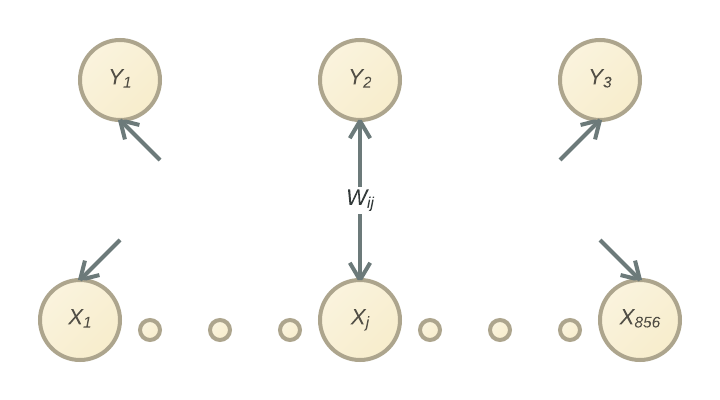
\includegraphics[width=0.7\linewidth]{img/parte1-modelo.png}

	\caption{Modelo de red}
\end{figure}

